\documentclass[11pt,a4paper]{article}

\usepackage[utf8]{inputenc} 
\usepackage[T1]{fontenc} 
\usepackage{lmodern}
\usepackage[margin=2cm]{geometry}
\usepackage[german]{babel}

\setlength{\parindent}{0pt}
\setlength{\parskip}{1ex plus 0.5ex minus 0.5ex}

\usepackage{amsmath} 
\usepackage{graphicx} 
\usepackage{booktabs}
\usepackage[colorlinks]{hyperref}
\usepackage{nicefrac}

\begin{document}

{
\centering 
\large 
Physiklabor für Anf\"anger*innen \\
Ferienpraktikum im Sommersemester 2018 \\[4mm]
\textbf{\LARGE 
Versuch 04: Dichte und Oberflächenspannung
} \\[3mm]
(durchgef\"uhrt am 07.09.2018 bei Daniel Bartle) \\
Andréz Gockel, Patrick M\"unnich\\
\today \\[10mm]
}

\section{Ziel des Versuchs}

Der Versuch ist in zwei Teile geteilt, welche dazu dienen, grundlegende Eigenschaften von Fl\"ussigkeiten experimentell zu bestimmen. Im Teil A bestimmt man die Dichte von Wasser und einer unbekannten Fl\"ussigkeit mithilfe einer Jollyschen Federwaage. Im Teil B bestimmt man die Oberfl\"achen\-spannung von Wasser durch Messen der Abrisskraft mithilfe eines Torsionskraftmessers.

%%%%% Auswertung und Fehleranalyse

\section{Auswertung und Fehleranalyse}


\subsection{Teil A - Dichte}

\subsubsection{Aufgabenstellung}
Mit Hilfe der Jollyschen Federwaage sind zu bestimmen
\begin{enumerate}
\item{die Dichte eines geometrisch einfach gestalteten K\"orpers, wobei ein Vergleich mit den aus den
geometrischen Abmessungen und dem Gewicht des K\"orpers gewonnenem Wert durchzuf\"uhren
ist,}
\item{die Dichte einer unbekannten Fl\"ussigkeit.}
\end{enumerate}

\subsubsection{Auswertung}

Zur ersten Aufgabe:\\
Die Messungen wurden mit einer Metallkugel durchgef\"uhrt mit einem Durch\-messer von $d=(1.2\pm0.03)$cm und einer Masse von $m=(7.03\pm0.005)$g. Mit der Formel f\"ur das Volumen, $V=\frac{\pi}{6}d^3$, und f\"ur die Dichte, $\rho=\frac{m}{V}$, ergibt sich ein Wert von $(7810\pm550)\mathrm{\frac{kg}{m^3}}$. Hierbei wurde der Fehler \"uber die Potenz\-formel des Gau\ss 'schen Fehlerfortpflanzungsgesetzes ($\delta V=\frac{\Delta V}{V},\ \delta V=3\delta d$) bei Vernachl\"assigung des Fehlers der Masse bestimmt.\\

$$
 \begin{array}{ll}
 	 \textrm{In Wasser}: \\ \textrm{werte in mm} \\ \textrm{Unsicherheit: $\pm 0.1$mm}
 \end{array}
%\rowcolors{2}{gray!10}{white}
\noindent%
\begin{tabular}{|l | ccccc|}
\hline
Messung & 1 & 2 & 3 & 4 & 5\\
\hline
Ruhelage $x_0$ & 441 & 479 & 473 & 463 & 468\\
Nicht eingetaucht $x_1$ & 414 & 453 & 447 & 436 & 440\\
Eingetaucht $x_2$ & 417 & 456 & 450 & 439 & 443\\
\hline
\end{tabular} \phantom{\begin{array}{ll}
 	 \textrm{In Wasser}: \\ \textrm{werte in mm} \\ \textrm{Unsicherheit: $\pm 0.1$mm}
 \end{array}
}$$

F\"ur das Dichteverh\"altniss gilt:\\

\begin{equation}
\frac{\rho}{\rho_{Fl}} = \frac{F_G}{F_G - F_{G'}}\label{eq2}
\end{equation}

\begin{equation}
F = -k(x-x_0)\mathrm{,}\label{eq3}
\end{equation}

wobei die Gr\"o\ss en in (\ref{eq2})
\begin{itemize}
  \item $\rho$ und $\rho_{Fl}$ jeweils die Dichten von dem K\"orper und der Fl\"ussigkeit.
  \item $F_G$ die Gewichtskraft des K\"orpers in Luft.
  \item $F_{G'}$ die Gewichtskraft des K\"orpers in einer Fl\"ussigkeit.
\end{itemize}

und in (\ref{eq3})
\begin{itemize}
  \item $F$ die Federkraft
  \item $k$ die Federkonstante
  \item $x_0$ die Ruhelage der Waage
  \item $x$ die Auslenkung der Waage sind.
\end{itemize}

Daraus ergibt sich f\"ur die Dichte mit den Auslenkungen $x_1$ Objekt in Luft und $x_2$ Objekt in Fl\"ussigkeit:
\begin{equation}
\rho=\rho_{Fl}\frac{x_1-x_0}{x_1-x_2}.\label{eq1}
\end{equation}
F\"ur unsere Messwerte aus Tabelle 1 erhalten wir

%NICEFRAC
$$\begin{tabular}{|c|c|c|c|c|c|}
\hline
\textrm{Messung} & 1 & 2 & 3 & 4 & 5\\
\hline
$\textrm{Dichte }\rho\left[\nicefrac{\textrm{kg}}{\textrm{m}^3}\right]$ & $8982\pm4260$ & $8649\pm4104$ & $8649\pm4104$ & $8982\pm4260$ & $9314\pm4416$\\
\hline
\end{tabular} $$

Der Mittelwert unserer Messung betr\"agt also $\rho=(8900\pm1800)\mathrm{\frac{kg}{m^3}}$. Diese Rechnungen wurden mit dem \textit{uncertainties} Paket in Python durchgef\"uhrt. Siehe Abbildung (\ref{ab1}).

\begin{figure}[p]
\centering
\fbox{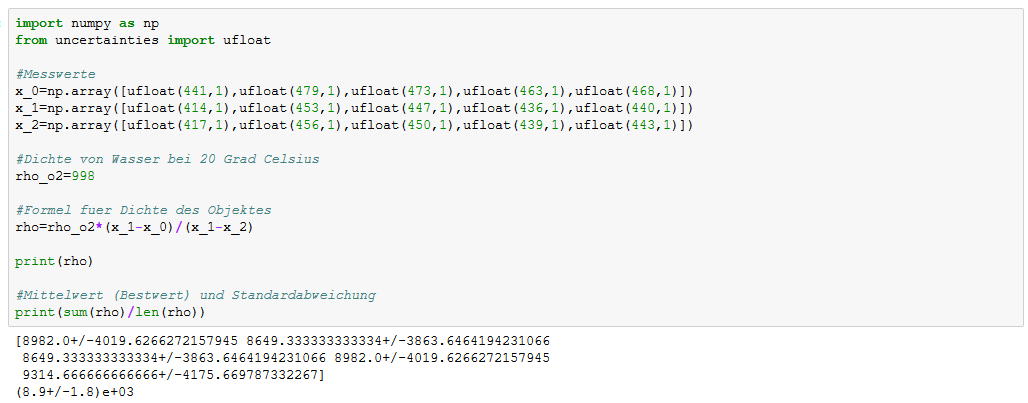
\includegraphics[width=0.8\textwidth]{/home/a/Documents/uni/AP1/git/Praktikum-A1/4/Rechnung_1.PNG}\label{ab1}}
\caption{Rechnungen mit Python und $uncertainties$ Paket.}
\label{abbildung}
\end{figure}

Der Fehler der Messung mit der Jollyschen Waage ist aufgrund des gro\ss en Dichteunterschieds zwischen dem Metall und der Fl\"ussigkeit so gro\ss. Dadurch ist die Auftriebskraft im Vergleich zur Gewichtskraft der Kugel klein und man erh\"alt im Nenner von (\ref{eq1}) die Differenz zweier nahezu gleichen Messwerte, deren Fehler dann gro\ss\ ist.\\

Zur zweiten Aufgabe:\\
Die Rechnungen wurden mit den Messwerten aus dem ersten Aufgabenteil durchgef\"uhrt und es wurde die gleiche Apparatur verwendet. Als Wert f\"ur die Dichte des K\"orpers wurde der Mittelwert auf dem ersten Aufgabenteil genutzt. Die Formel (\ref{eq1}) wurde zu
\begin{equation}
\rho_{Fl}=\rho\frac{x_1-x_2}{x_1-x_0}\label{eq4}
\end{equation}
umgestellt.

F\"ur die unbekannte Fl\"ussigkeit wurde gemessen:

$$
 \begin{array}{ll}
 	 \textrm{In Fl\"ussigkeit}: \\ \textrm{werte in mm} \\ \textrm{Unsicherheit: $\pm 0.1$mm}
 \end{array}
%\rowcolors{2}{gray!10}{white}
\noindent%
\begin{tabular}{|l | cccc|}
\hline
Messung & 1 & 2 & 3 & 4\\
\hline
Ruhelage $x_0$ & 449 & 466 & 440 & 482\\
Nicht eingetaucht $x_1$ & 424 & 438 & 414 & 455\\
Eingetaucht $x_2$ & 427 & 441 & 417 & 458\\
\hline
\end{tabular} \phantom{\begin{array}{ll}
 	 \textrm{In Fl\"ussigkeit}: \\ \textrm{werte in mm} \\ \textrm{Unsicherheit: $\pm 0.1$mm}
 \end{array}
}$$

Mit (\ref{eq4}) ergibt sich dann:

%NICEFRAC
$$\begin{tabular}{|c|c|c|c|c|c|}
\hline
\textrm{Messung} & 1 & 2 & 3 & 4\\
\hline
$\textrm{Dichte }\rho\left[\nicefrac{\textrm{kg}}{\textrm{m}^3}\right]$ & $1068\pm523$ & $953\pm469$ & $1026\pm504$ & $989\pm486$\\
\hline
\end{tabular} $$

Hier ist der Mittelwert dann $\rho_{Fl}=(1010\pm300)\mathrm{\frac{kg}{m^3}}$. Die Rechnungen wurden hier wieder mit dem $uncertainties$ Paket in Python durchgef\"uhrt. Siehe Abbildung (\ref{ab2}).

\begin{figure}[p]
\centering
\fbox{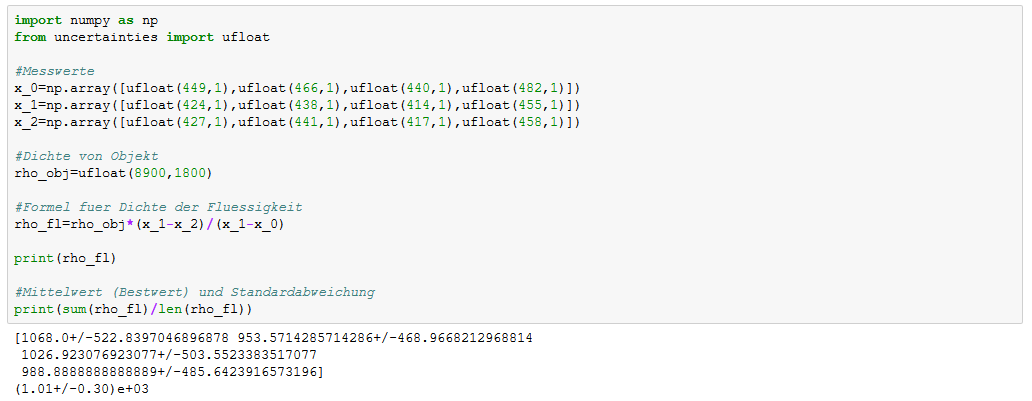
\includegraphics[width=0.8\textwidth]{/home/a/Documents/uni/AP1/git/Praktikum-A1/4/Rechnung_2.PNG}\label{ab2}}
\caption{Rechnungen mit Python und $uncertainties$ Paket.}
\label{abbildung}
\end{figure}

\subsubsection{Unsicherheitsvergleich mit Streuung}

Aus den 5 bzw. 4 Einzelwerten der beiden Messungen ergeben sich folgende Streuungen:\\

$$s_\rho=279,\ \mathrm{\nicefrac{kg}{m^3}},\ s_{\rho_{Fl}}=49.1,\ \mathrm{\nicefrac{kg}{m^3}}$$

Diese Werte sind erheblich kleiner als erwartet. Der Grund daf\"ur k\"onnte bei einer zu groben Absch\"atzung der Messungenauigkeit oder aufgrund der geringen Anzahl an Einzelmessungen (5 bzw. 4) liegen.\\

Geht man von einer halb so gro\ss en Messungenauigkeit aus, so erh\"alt man Fehlerabsch\"atzungen von etwa 2000 $\mathrm{\nicefrac{kg}{m^3}}$, was immer noch nicht konsistent mit der Absch\"atzung mittels $s_\rho$ ist. Daher m\"ussen wir davon ausgehen, dass die kleinen Werte von $s_\rho\textrm{ und}\ s_{\rho_{Fl}}$ durch die geringe Anzahl an Einzelmessungen zustande gekommen sind.\\

Aus den Unsicherheiten der Einzelmessungen ergeben sich Standardabweichungen des Mittelwerts von:\\
\[
s_{\overline{\rho}}=(3987\pm125)\nicefrac{kg}{m^3},\ 
s_{\overline{\rho_{Fl}}}=(505\pm25)\nicefrac{kg}{m^3}
\]

Bei der Messreihe mit der unbekannten Fl\"ussigkeit gibt es einen systematischen Fehler aufgrund der verwendeten gemessenen Dichte des K\"orpers, die unter umst\"anden zu gro\ss\ oder zu klein gesch\"atzt wurde und als Referenz dient.

\subsection{Teil B - Oberfl\"achenspannung}

Die Oberfl\"achenspannung von Wasser und Ethanol wurde mit der Abrei\ss methode gemessen. F\"ur diese gilt:

\begin{equation}
\sigma=\frac{F_(s_{max})}{2l}\label{eqo}
\end{equation}

$$\begin{tabular}{|c|c|c|c|c|c|c|c|}
\hline
\textrm{H\"ohe }$[mm]$ & 2 & 4 & 5 & 8 & 9 & 10\\
\hline
$\textrm{Kraft }[mN]$ & $0.26\pm0.03$ & $0.33\pm0.03$ & $1.25\pm0.03$ & $3.9\pm0.03$ & $4.75\pm0.03$\\
\hline
\end{tabular} $$\label{tabow}

Die L\"ange $l$ des Drahts betr\"agt $2.63\pm0.03$ cm. Die Messwerte befinden sich in Tabelle (\ref{tabow}) f\"ur Wasser und (\ref{taboe}) f\"ur Ethanol. Deren Graphische Darstellungen in den Graphiken (\ref{ab3}) und (\ref{ab4}). Die Sigmoidfunktion $$d\times\frac{1}{1+\exp(-c\times(x-a))}+b$$ wurde mit der curve\_fit Funktion von Python an die Messpunkte angepasst. Aus den Graphiken lesen wir folgende Werte f\"ur $F_{s_{max}}$ ab:

TABELLE
%5.16, 4.75, 

Die Fehler wurden durch Streuung der Messpunkte um die angepassten Kurven abgesch\"atzt.

Mit der Formel (\ref{eqo}) ergibt sich f\"ur die Oberfl\"achenspannung 

TABELLE

MITTELWERT

\begin{figure}[p]
\centering
\fbox{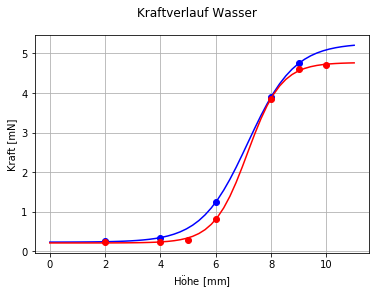
\includegraphics[width=0.8\textwidth]{/home/a/Documents/uni/AP1/git/Praktikum-A1/4/Wasser.png}\label{ab3}}
\caption{Verlauf der Kraft $F$ als Funktion der Position $x$ beim Herausziehen des B\"ugels aus der Fl\"ussigkeit.}
\label{abbildung}
\end{figure}

\begin{figure}[p]
\centering
\fbox{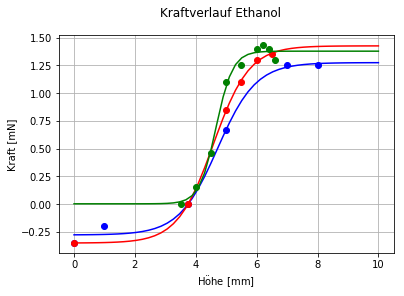
\includegraphics[width=0.8\textwidth]{/home/a/Documents/uni/AP1/git/Praktikum-A1/4/Fluessigkeit.png}\label{ab4}}
\caption{Verlauf der Kraft $F$ als Funktion der Position $x$ beim Herausziehen des B\"ugels aus der Fl\"ussigkeit.}
\label{abbildung}
\end{figure}

%%%%% Anhang

\section{Anhang: Tabellen und Diagramme}

Tabelle \ref{tabelle} wurde mit der Umgebung "`tabular"' erzeugt
und mit der Umgebung "`table"' eingebunden.  

%\begin{table}[p]
%\centering
%\begin{tabular*}{0.99\textwidth}{@{\extracolsep{\fill}}cccccc}
%\toprule
% $x$ & $u_x$ &  $y$  &  $u_y$ &  $y^2$  &  $2 y u_y$  \\
% m & m &  s & s &  s$^2$ & s$^2$  \\
%\midrule
%  0,16 & 0,01 & 0,686 & 0,029 & 0,47 & 0,040 \\
%  0,33 & 0,01 & 1,046 & 0,031 & 1,09 & 0,065  \\
%  0,52 & 0,01 & 1,381 & 0,026 & 1,91 & 0,072  \\
%  0,69 & 0,01 & 1,607 & 0,021 & 2,58 & 0,067  \\
%  0,85 & 0,01 & 1,785 & 0,022 & 3,19 & 0,079  \\	
%\bottomrule
%\end{tabular*}
%\caption{Eine Tabellenunterschrift.}
%\label{tabelle}
%\end{table}


%\begin{figure}[p]
%\centering
%\includegraphics[width=0.8\textwidth]{bild.png}
%\caption{Eine Bildunterschrift.}
%\label{abbildung}
%\end{figure}



\end{document}
%%%%%%%%%%%%%%%%%%%%%%%%%%%%%%%%%%%%%%%%%